\documentclass[a4paper,12pt]{article}

\usepackage[utf8]{inputenc}
\usepackage[french]{babel}
\usepackage{graphicx}
\graphicspath{{./img/}}
\usepackage{xcolor}
\usepackage{amsmath, amssymb}
\usepackage[left=3cm,right=3cm,top=2cm,bottom=2cm]{geometry}
\usepackage{url}
\usepackage{listings}
\usepackage{fancybox}
\definecolor{darkWhite}{rgb}{1.00,1.00,1.00}

\lstset{
aboveskip=3mm,
belowskip=2mm,
backgroundcolor=\color{darkWhite},
%basicstyle=\footnotesize,
breakatwhitespace=false,
captionpos=b,
commentstyle=\color{black},
deletekeywords={...},
escapeinside={\%*}{*)},
extendedchars=true,
keepspaces=true,
%keywordstyle=\color{blue},
language=C,
literate=
{²}{{\textsuperscript{2}}}1
{⁴}{{\textsuperscript{4}}}1
{⁶}{{\textsuperscript{6}}}1
{⁸}{{\textsuperscript{8}}}1
{€}{{\euro{}}}1
{é}{{\'e}}1
{è}{{\`{e}}}1
{ê}{{\^{e}}}1
{ë}{{\¨{e}}}1
{É}{{\'{E}}}1
{Ê}{{\^{E}}}1
{û}{{\^{u}}}1
{ù}{{\`{u}}}1
{â}{{\^{a}}}1
{à}{{\`{a}}}1
{á}{{\'{a}}}1
{ã}{{\~{a}}}1
{Á}{{\'{A}}}1
{Â}{{\^{A}}}1
{Ã}{{\~{A}}}1
{ç}{{\c{c}}}1
{Ç}{{\c{C}}}1
{õ}{{\~{o}}}1
{ó}{{\'{o}}}1
{ô}{{\^{o}}}1
{Õ}{{\~{O}}}1
{Ó}{{\'{O}}}1
{Ô}{{\^{O}}}1
{î}{{\^{i}}}1
{Î}{{\^{I}}}1
{í}{{\'{i}}}1
{Í}{{\~{Í}}}1,
morekeywords={*,...},
numbers=left,
numbersep=10pt,
numberstyle=\tiny\color{black},
rulecolor=\color{black},
showspaces=false,
%showstringspaces=false,
showtabs=false,
stepnumber=1,
stringstyle=\color{darkgray},
tabsize=4,
title=\lstname,
%---efface
showstringspaces=false,
basicstyle=\footnotesize\ttfamily,
keywordstyle=\bfseries\color{green!40!black},
commentstyle=\itshape\color{purple!40!black},
identifierstyle=\color{black},
stringstyle=\color{orange},
}


\usepackage[french]{babel}

\begin{document}


\includegraphics[width=0.3\textwidth]{enseirb-matmeca.png}
\begin{center}
\vspace{2\baselineskip}
  \Huge
  \textcolor{darkgray}{\textbf{Atomic Teddy Investors}}\\
\vspace{4\baselineskip}
\large
Projet réalisé par \\
\Huge
\vspace{3\baselineskip}
Mougou Yassine\\
Moussa Guimba Mamadou\\
\vspace{3\baselineskip}
\large
Groupe 7340\\
\vspace{5\baselineskip}
Année 2019/2020
\end{center}
\large

\normalsize
\newpage 
\section{Introduction}

Dans le cadre du projet de première année, filière informatique, il nous est proposé de mettre en application nos compétences en programmation en mettant en place un système de jeu, écrit en langage C, portant sur le marché des changes et faisant intervenir des ours.

  \subsection{Contexte}
Aussi comique qu'il puisse paraître, dans ce jeu des ours de la Sicile se mettent dans la pratique d’activités humaines et finissent par s’infiltrer dans le monde du marché économique. Leur objectif principal est la quête du miel. C’est dans ce contexte que se situe le projet où il est demandé spécifiquement de mettre en place un système de jeu permettant aux ours d’explorer les places du marché de la Sicile et d’effectuer un certain nombre d’échanges leur permettant d’atteindre leur but.

  \subsection{Problématique}
Le miel étant la cible principale des ours, toute ressource possédée a sa valeur en équivalent miel. Ainsi le but de ce jeu est d'établir un certain nombre de stratégies qui permettent aux ours de découvrir les marchés de la Sicile et de viser leur idéal. \\
Pour cela, il nous faut une bonne hiérarchisation du jeu et des outils pour bien gérer notre projet.

\section{Cadre de travail}
\paragraph{}
Afin de mener à bien notre travail, nous avions eu recours au logiciel de gestion de version GIT. Chacun des membres ayant son propre dépôt de travail local, ce logiciel nous permet de décomposer le travail, de garder une trace des modifications personnelles apportées et permet ainsi de récuperer l'ancien état de nos données.

\paragraph{}
Au fur et à mesure de l'avancement de notre projet, nous sommes amenés à communiquer une révision au dépôt distant qui est celui de la forge de l'école, ce qui rend le travail recupérable par l'autre membre du groupe. Sur la forge, se trouve un ensemble de tests nous permettant de vérifier le fonctionnement de notre code et ainsi valider les tâches qui nous sont demandées.

\section{Structure du projet}

\paragraph{}
Dans le marché de la Sicile s'échange un ensemble de ressources dont principalement le miel. Afin de rendre les échanges plus faciles, chaque ours appelé egalement \textbf{Teddy}, dispose d'un portefeuille où stocker ses ressources et chaque ressource a une valeur de réference qui est sa valeur en équivalent-miel.\\
Pour éffectuer les échanges, des places d'échanges dites \textbf{stockex} sont à la disposition des ours sur toute la côte. Au niveau de chaque place, il existe un certain nombre de transactions où s'échangent differentes ressources.
Ainsi, pour jouer, les ours sont placés dans une queue où la priorité revient à l'ours ayant passé le moins de temps à éffectuer une transaction.

 \subsection{Les structures de base}
Plusieurs structures sont définies pour représenter les différentes données:
\begin{itemize}
\item Les ours sont représentés par une structure nommée teddy, et figure dans un
fichier \textcolor{darkgray}{\textbf{teddy.h}}. Un ours est caractérisé par son nom, son portefeuille et sa priorité.
\begin{lstlisting}[language={C},captionpos=b, frame=single, caption = Structure Teddy]
struct teddy {
  char name[MAX_TEDDY_NAME + 1]; 
  struct wallet w;  
  int priority;
  int time ;       // the time when a teddy is called to play
  int count_stockex_done; // the number of stockex he visited
  const struct stockex* stockex_done[MAX_STOCKEX];
  const struct stockex* accessible_stockex;  //the next stockex
                                             // he'll visit
};
\end{lstlisting}

\item les places d'échanges et transactions sont également représentées respectivement par \textbf{struct stockex} et \textbf{struct transac}. Une place d'échange contient plusieurs transactions qui se caractérisent à leur tour par le portefeuille de ressources achetées et celui de ressources vendues. 
\begin{lstlisting}[language={C},captionpos=b, frame=single, caption= Structures transac et stockex]
struct transac {
  int index_stockex;  // the index of the stockex 
                     // where the transaction is made
  int index_accessible_stockex; //index of the accessible
                             // stockex after this transaction
  struct wallet in_wallet; 
  struct wallet out_wallet; 
};

struct stockex {
  char name[MAX_STRING + 1];
  int count_transac;       
  struct transac transaction[MAX_TRANSAC];
};
\end{lstlisting}
\emph{Struct wallet} est la structure qui représente les portefeuilles.

\item On utilise le type enum pour l'énumeration des différentes resssources. A titre d'exemple on peut avoir comme ressources:
\begin{lstlisting}[language={C},captionpos=b, frame=single, caption = Enumération des ressources]
enum good {
           HONEY,           // Always first
           MONKEY_WRENCH,
           OUTBOARD_MOTOR,
           MAX_GOOD = 20,        // Always last
           ERROR_GOOD = -1, // Always -1
};
\end{lstlisting}

\item La file de priorité où sont placés les ours est définit par \textbf{struct queue} et contient un \textbf{tableau} de \textbf{struct} teddy.
\newpage
\begin{lstlisting}[language={C},captionpos=b, frame=single, caption = Structure Queue]
struct queue {
  int count_teddy;
  struct teddy ours[MAX_TEDDY];
};
\end{lstlisting}

\end{itemize}
Nous expliquerons le rôle des autres données des différentes structures dans la suite de ce rapport.

  \subsection{Les fichiers de code}

Vu que le jeu fait intervenir plusieurs thèmes, pour l'écriture du code, il est nécessaire d'avoir deux types de fichiers: les fichiers \textbf{.c} et \textbf{.h}. Pour chaque fichier.c, il y a son équivalent .h qui contient les prototypes des fonctions. L'intérêt d'un fichier .h c'est que lorsqu'on appellera une fonction située dans un fichier par exemple objet.c depuis un autre fichier boite.c, nous aurons besoin d'inclure dans boite.c le fichier objet.h. \\
Alors pour ce jeu nous avions besoin de plusieurs fichiers à savoir:
\newline
\begin{itemize}
\item \textcolor{darkgray}{\textbf{good.[ch]}} pour la gestion des ressources;
\item \textcolor{darkgray}{\textbf{stockex.[ch]}} pour celle des places d'échanges et des transactions;
\item \textcolor{darkgray}{\textbf{queue.[ch]}} pour les fonctions en rapport avec la file à priorité;
\item \textcolor{darkgray}{\textbf{teddy.h}} pour la struture des ours;
\item \textcolor{darkgray}{\textbf{define.h}} où sont définies nos variables de substitutions.
\item \textcolor{darkgray}{\textbf{project-0.c}} où est implémentée la boucle de jeu;
\item \textcolor{darkgray}{\textbf{test-0.c}} où sont réalisés les tests des différentes fonctions qui sont implémentés dans les différents fichiers .c.
\end{itemize}

\paragraph{}
Pour une bonne gestion du projet, le jeu est décomposé en plusieurs parties appélées achievement. Et chaque partie n'apporte qu'une petite modification de code à celle qui la précéde. Et donc notre dépôt doit être structuré d'une manière à avoir un répertoire pour chaque partie. 
Tout répertoire contient:
\newline
\begin{itemize}
\item un fichier \textbf{Makefile} qui nous permet avec la commande "make" de compiler nos fichier.c et de vérifier nos tests; 
\item un sous-répertoire \textbf{src} qui contient les fichiers cités ci-dessus; 
\item et un sous-répertoire \textbf{tst} qui contient le fichier \textcolor{darkgray}{\textbf{test-0.c}}.
\end{itemize}

Le schéma suivant résume tout ce qui précéde.
\newpage

\begin{figure}[!h]
  \centering
  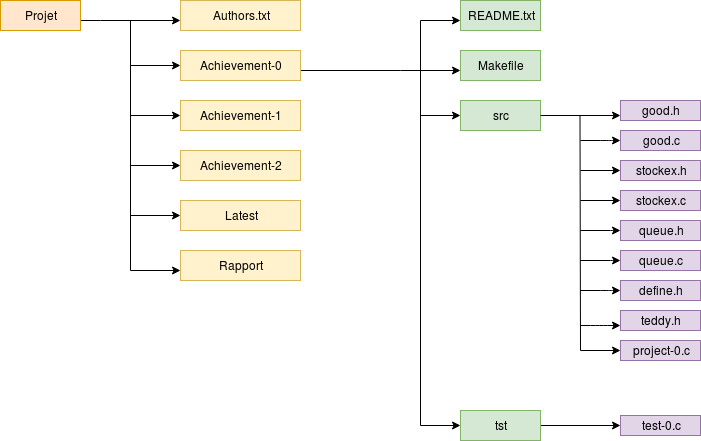
\includegraphics[width=1\textwidth]{StructureRep.png}
  \caption{La structure des répertoires du projet}
  \label{fig:rep}
\end{figure}

  \subsection{Le fichier Makefile}
Dans tous les répertoires se trouve un fichier Makefile qui permet de compiler les différents fichiers de code et de lancer les exécutables. Il est constitué de plusieurs cibles qui seront dans notre cas les exécutables \textcolor{darkgray}{\textbf{test}}, \textcolor{darkgray}{\textbf{project}} et \textcolor{darkgray}{\textbf{clean}}. Une cible peut posséder à son tour une liste de prérequis qui doivent être atteints avant son exécution. Ces prérequis ne sont autres que les fichiers objets \textbf{.o} qui à leur tour ont une dépendance avec leur fichier \textbf{.c} respectifs.
\begin{itemize}
\item la cible project permet la création de l'exécutable project, et cela après compilation des fichiers \textcolor{darkgray}{\textbf{good.c, stockex.c, queue.c}} et \textcolor{darkgray}{\textbf{project-0.c}}.
\item de même la cible test permet de générer l'exécutable test;
\item  la cible clean permet de supprimer les exécutables et les prérequis.
\end{itemize}
Le schéma suivant résume le fonctionnement du Makefile. 
\begin{figure}[!h]
  \centering
  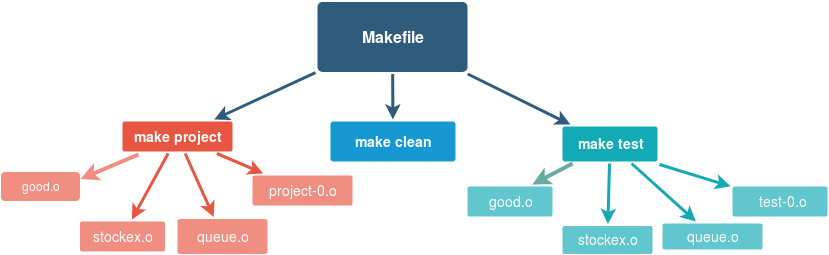
\includegraphics[width=1\textwidth]{makefile.png}
  \caption{Présentation du Makefile}
  \label{fig:make}
\end{figure}

\section{Gestion du jeu}
  \subsection{La file à priorité}
Au début du jeu, les ours sont placés dans la queue en fonction de leur priorité. Rappelons que la priorité revient à l'ours ayant passé le moins de temps à effectuer une transaction. Alors pour la gestion de cette file, nous avons besoin de plusieurs fonctions à savoir:
\begin{itemize}

\item[$-$] une fonction struct queue \emph{\textbf{init\_queue}}(), qui initialise la \textbf{queue}. Cette fonction figure dans \emph{queue.c} et est de compléxité en temps linéaire \textbf{O(n)} où \textbf{n} est le nombre de teddy;
\newline
\item[$-$] les fonctions \emph{\textbf{queue\_\_pop}} et \emph{\textbf{queue\_\_push}}; la première retourne et supprime l'ours prioritaire de la queue et la seconde remet un ours après avoir joué avec sa nouvelle priorité.\\
Il y'avait plusieurs choix pour la représentation de la queue. Nous avons opté pour un tableau de struct teddy. Cela rendait plus simple l'implémentations des deux fonctions.
\newline
\begin{itemize}

\item [$\ast$] Pour la fonction \emph{\textbf{queue\_\_push}}, nous avions utilisé une fonction auxiliaire \textbf{int index\_of\_teddy} qui nous permet de connaitre l'indice où doit être placé l'ours avec sa nouvelle priorité. Pour cela on a utilisé la méthode du \textbf{tri par insertion} pour l'insérer car il faut savoir dès le début du jeu, que chaque ours débute avec la priorité 0 ; ce qui fait de notre tableau un tableau trié. \\
Il arrive par contre que certains ours dans la queue possèdent la même priorité que celui qui a joué; il serait donc injuste de le placer avant les autres n'ayant pas encore joué. Pour cela, on a implémenté une fonction \textbf{int count\_same\_priority} qui retourne le nombre d'ours ayant la même priorité que celui qui joue. Ainsi l'ours sera placé après ces derniers pour pouvoir leur donner la chance de passer.
\newline
\item [$\ast$] En ce qui concerne la fonction \emph{\textbf{queue\_\_pop}}, l'ours prioritaire est celui qui est placé au début du tableau. Mais puisque la fonction doit le retourner et le supprimer de la queue, il suffit juste de faire avancer les autres ours, de placer l'ours prioritaire à la fin du tableau, de décrémenter le compteur de teddy et de retourner un pointeur vers ce teddy.
Ces fonctions sont toutes de compléxité en temps linéaire et en espace constante.
\newline
\end{itemize}
\end{itemize}

  \subsection{La boucle de jeu}

La boucle de jeu est implémentée dans le fichier \textbf{project-0.c} et pour la faire tourner, il est possible de choisir le nombre de joueurs et le nombre de tours. Pour cela, on fait appel à la fonction \textbf{getopt} qui analyse les arguments passés en ligne de commande. Alors la commande pour faire tourner le jeu est la suivante: ./project -n x -m y -s z où :
\begin{itemize}
\item l'option -n x désigne le nombre de joueurs x;
\item l'option -m y est pour le choix du nombre de tours y;
\item et l'option -s z pour initialiser le génerateur aléatoire à z.
\end{itemize}
    \subsubsection{La stratégie aléatoire}

Pour le moment, partons du plus simple; les ours se dirigent tous vers la place d’échange initiale fournie par la fonction \textbf{starting\_stockex}() implémentée dans le fichier \emph{stockex.c}. Lors du passage de l'ours, il choisit aléatoirement une transaction et décide du nombre de fois où il désire effectuer cette transaction.  S'il arrive que l'ours ne dispose pas de ressources nécessaires pour l'effectuer, il passe son tour pendant une unité de temps. La durée de la partie est de 1000. \\
Pour cela nous avons besoin d'autres fonctions que l'on ajoute dans \emph{queue.c} à savoir:
\newline
\begin{itemize}
\item[$-$] Une fonction \emph{\textbf{int active\_teddy\_play}} qui fait jouer \textbf{N} fois l'ours sur la transaction \textbf{n} de la place d'échange et retourne le temps passé sur cette transaction; \textbf{N} et \textbf{n} sont choisit de manière aléatoire. Cependant, il serait intéressant de savoir le maximum de transaction que l'ours peut effectuer et de prendre aléatoirement entre 1 et ce maximum. Pour cela, nous avons implémenté une fonction \emph{\textbf{max\_transaction}} qui retourne le nombre maximum de fois que le teddy peut faire son échange. Cette fonction est dans le pire des cas, de compléxité en temps linéaire et en espace constante.
\newline
\item[$-$] Une fonction \emph{\textbf{void display\_results}}(struct queue q) qui affiche l'ours gagnant, celui qui posséde le maximum d'équivalent en miel.
\newline
\end{itemize}


\paragraph{}
Ainsi le principe algorithmique de la boucle de jeu est le suivant:\\

\fbox{\parbox{\textwidth}{
\textbf{Tant que } le temps global est inférieur à la durée de la partie \textbf{faire:} \\

\indent faire sortir l'ours prioritaire de la queue;\\
\indent faire jouer l'ours;\\
\indent remettre l'ours dans la queue avec sa nouvelle priorité;\\
\indent incrémenter le temps global;\\

\textbf{Fin tant que} \\
\textbf{Afficher} le teddy gagnant 
}}

\paragraph{}
Il est évident qu'avec une seule place d'échange le jeu devient de plus en plus ennuyant. C'est la raison pour laquelle, dorénavant, il existe plusieurs places d'échanges qui proposent différents types de transactions. À présent l'objectif de tout ours est de visiter toutes les places d'échanges. Étant donné que ces dernières ne sont pas accessibles immédiatement, chaque transaction donne accées à une nouvelle place d'échange. Alors pour ordonner le jeu, tous les ours débutent avec la place d'échange initiale que fournit la fonction \textbf{starting\_stockex}().\\
On placera toutes les places d'échanges disponibles dans le jeu, dans un tableau \textbf{tab\_stockex} que l'on définit statiquement dans stockex.c. Ainsi, nous avons besoin de nouvelles fonctions dans le fichier \textcolor{darkgray}{\textbf{stockex.c}}:
\newline
\begin{itemize}
\item la fonction \emph{\textbf{transac\_\_stockex}} qui renvoit un pointeur vers la place d'échange où est effectué une transaction passée en paramètre;
\item et la fonction \emph{\textbf{transac\_\_next\_stockex}} qui renvoit un pointeur vers la place d'échange accessible après avoir effectué une transaction passée en paramètre.
\newline
\end{itemize}
Ces fonctions comme toutes les autres fonctions définies dans \textbf{stockex.c} sont de compléxité, en temps et en espace, constante. 

\paragraph{}
L'objectif de l'ours étant de visiter toutes les places d'échanges, arrivé à une place, il doit choisir une transaction lui permettant d'accéder à une autre qu'il n'a jamais exploré. S'il arrive à tout visiter, l'ours choisira la transaction aléatoirement. D'où le rôle des deux données dans la struture teddy:
\newline
\begin{itemize}
\item \textbf{const struct stockex* accessible\_stockex} qui contient le stockex accessible à l'ours lors de son prochain passage. 
\item \textbf{const struct stockex* stockex\_done[MAX\_STOCKEX]} un tableau qui sera rempli par des pointeurs vers des places déjà visitées par l'ours en question. \\
\end{itemize} 

Ainsi que ceux de la structure transac:
\begin{itemize}
\item \emph{\textbf{int index\_stockex}}, l'indice dans \textbf{tab\_stockex} de la place d'échange où est effectué la transaction;
\item \emph{\textbf{int index\_accessible\_stockex}}, l'indice dans \textbf{tab\_stockex} de la place d'échange accessible après avoir effectué la transaction.\\
\end{itemize}
Pour le choix de la transaction, nous avons ajouté une fonction \emph{\textbf{int index\_transac(const struct stockex* s, struct teddy* t)}} dans \emph{queue.c}. Cette fonction dans le pire des cas est de complexité en temps linéaire; c'est-à-dire lorsque la transaction qui avantage l'ours est la dernière dans le tableau des transactions.
\newline
\newline
Ainsi le principe algorithmique de la boucle de jeu est le suivant:\\

\fbox{\parbox{\textwidth}{
\noindent\textbf{Tant que } le temps global est inférieur à la durée de la partie \textbf{faire:} \\

  \indent faire sortir l'ours prioritaire de la queue;\\
  \indent l'orienter vers la place d'échange qui lui est accessible;\\
  \indent choisir la bonne transaction;\\
  \indent faire jouer l'ours;\\
  \indent remettre l'ours dans la queue avec sa nouvelle priorité;\\
  \indent incrémenter le temps global;\\

\textbf{Fin tant que} \\
\textbf{Afficher} le teddy gagnant
}}
\newline
\newline
Le schéma suivant résume la boucle de jeu:\\
Prenons à un instant donné par exemple, un ours \emph{Nest} de Priorité 1 qui n'a visité qu'une seule place nommée \emph{Catane} et qui a effectué une transaction qui le dirige vers \emph{Etna}.
\newpage
\begin{figure}[!h]
  \centering
  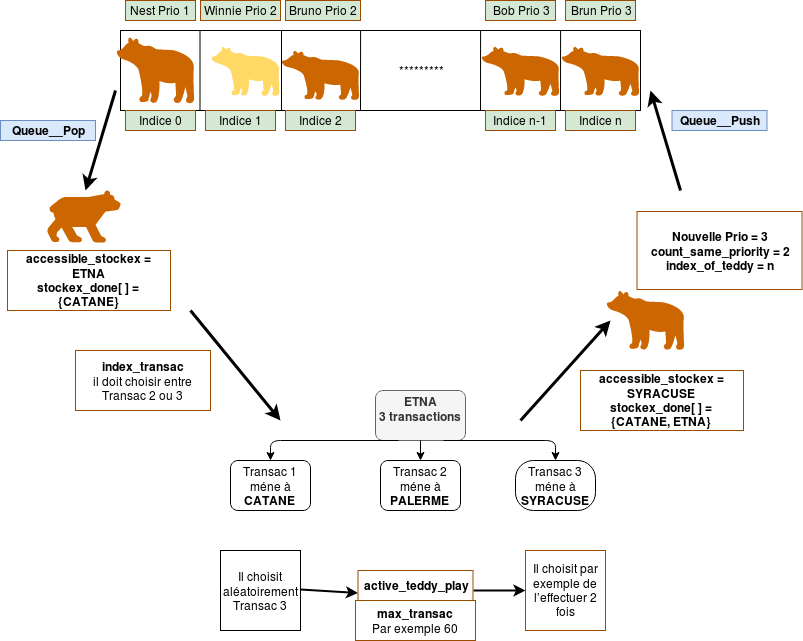
\includegraphics[width=1.2\textwidth]{strategie1.png}
  \caption{Déroulement du jeu}
  \label{fig:jeu}
\end{figure}

    \subsubsection{La deuxième strategie}
Maintenant qu'il existe plusieurs places dans le marché et que les ours arrivent à tout explorer, il serait intéressant d'attribuer à quelques ours des stratégies de jeu. En suivant ces stratégies, les ours gagneront plus en équivalent miel et tenteront de remporter la partie du jeu.
Pour cette partie, nous n'avons pu implémenté qu'une seule stratégie. 
N'oublions pas que les ours doivent visiter toutes les places d'échange; ainsi pour notre ours stratège, lorsqu'il arrive au niveau d'une place, il mémorisera toutes les transactions qui lui permettent de visiter de nouvelles places et ensuite il effectuera celle qui lui rapportera le maximum d'équivalent-miel. Après avoir tout visité, il choisit aléatoirement une place d'échange et effectue la meilleure transaction.\\
Nous avons appliqué cette stratégie aux deux premiers ours de la queue, et on remarque qu'après plusieurs exécutions de la boucle de jeu, ces derniers sont plus avantagés que les autres ours.\\
Pour les distinguer des autres joueurs, nous avons ajouté la fonction \emph{\textbf{strategy\_index
\_transac}} qui, comme \emph{\textbf{index\_transac}}, retourne l'indice la transaction qui arrange le plus les ours stratèges; et \emph{\textbf{choice\_of\_strategy}} qui attribue à chacun sa stratégie. Elles sont toutes dans le pire des cas de compléxité en temps linéaire.
\newline
\begin{lstlisting}[language={C},captionpos=b, frame=single, caption= Choix des stratégies]
int choice_of_strategy(const struct stockex* s, struct teddy* t)
{
  if((strcmp(t->name, "Teddy1") == 0) | 
  (strcmp(t->name, "Teddy2") == 0)){
    return strategy_index_transac(s, t);
  }
  else
    return index_transac(s, t);
}
\end{lstlisting}
Ainsi le principe de la boucle de jeu final est le suivant:
\begin{figure}[!h]
  \centering
  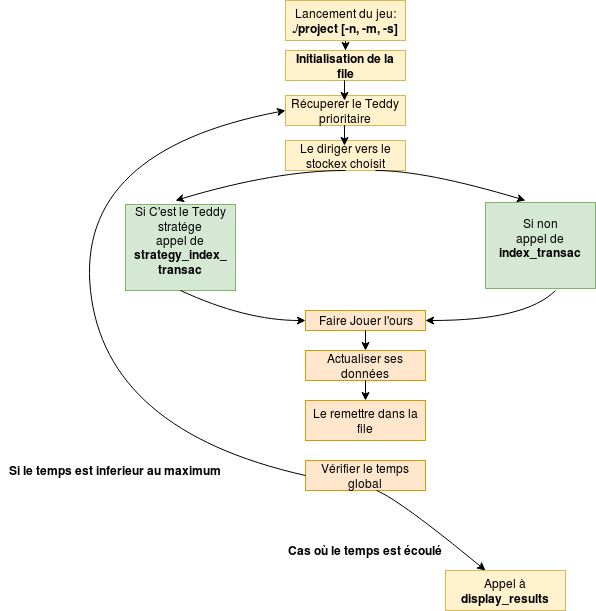
\includegraphics[width=1\textwidth]{BoucleJeuFinal.png}
  \caption{La boucle de jeu final}
  \label{fig:final}
\end{figure}

\section{Les fichiers de tests}

Les tests sont réalisés dans le fichier \textbf{test.c} de chaque achievement. Il contient une fonction \textbf{main()} et 3 autres fonctions:
\begin{itemize}

\item \textcolor{darkgray}{\textbf{test\_good()}} qui teste les fonctions du fichier good.c

\item \textcolor{darkgray}{\textbf{test\_stockex()}} qui teste les fonctions du fichier stockex.c

\item \textcolor{darkgray}{\textbf{test\_queue()}} qui teste toutes les fonctions en rapport avec la queue et la boucle de jeu.

\end{itemize}
Ces fonctions retournent 1 à la fin de l'éxecution et sont appelées par la fonction main() qui passe les tests. 
\begin{lstlisting}[language={C}, frame=single, caption = Les tests des différentes fonctions ]
int main()
{
  srand(time(NULL));
  if(test_good() != 0)
    printf("\n_____PASSED_TEST_____\n");
  if(test_stockex() != 0)
    printf("\n\n_____PASSED_TEST_____\n");
  if(test_queue() != 0)
    printf("\n_____PASSED_TEST_____\n");
 
}
\end{lstlisting}
 
\section{Conclusion}

\paragraph{}
L'objectif de ce projet était d'attribuer aux ours différentes stratégies de jeu. Partant d'une stratégie aléatoire à une stratégie bien déterminée, les ours ont pu jouer différemment et augmenter leur chance de gagner en visitant de nombreuses places d'échanges.\\
Néanmoins notre stratégie finale n'est pas la plus optimale. L'idéal pour l'ours stratége est de visiter successivement toutes les places d'échanges tout en choisissant la meilleure transaction. Après avoir tout visité, il refait le même trajet.

\end{document}